\documentclass[xcolor=dvipsnames,table,final]{beamer}
% \newcommand{\Sec}[3]{\section{\texorpdfstring{#1}{#2}}\label{#3}}
% \newcommand{\Subsec}[3]{\subsection{\texorpdfstring{#1}{#2}}\label{#3}}
\def\vrb#1{\texttt{\detokenize{#1}}}
\RequirePackage{pgfcore}
\usepackage{tau3mu.paper}
\usepackage{lmodern}
\usepackage{graphicx}
\usepackage{tikz}
\usepackage{hyperref}
\usepackage[nomessages]{fp}
\usepackage{pgfplots}
\usepackage{nicefrac,xcolor,verbatim,amsmath,bm,comment,url,epsfig,bm,wrapfig,Tabbing,wasysym,amssymb,axodraw,graphics,graphicx,appendix,multirow,epstopdf}
\usepackage[abs]{overpic}
\usepackage[english]{babel}
\usepackage[latin1]{inputenc}
\usepackage{times}
\usepackage{etex}
\usepackage{booktabs}
\usepackage[toc]{multitoc}
\usetikzlibrary{mindmap}
\usetikzlibrary{shapes,decorations,arrows,patterns,automata}
\usetikzlibrary{decorations.pathmorphing}
\usetikzlibrary{calc,decorations.pathreplacing,decorations.markings}
\usetikzlibrary{decorations.shapes}
\usetikzlibrary{decorations.text}
\usetikzlibrary{positioning}
\usetikzlibrary{scopes}
\usetikzlibrary{3d,calc}
\usepackage{tikz-3dplot}
\usetikzlibrary{shadings}
\usefonttheme{professionalfonts}
\mode<presentation>
{
	\usetheme{Montpellier}
	\usecolortheme{beaver}
	\setbeamercolor{title}{fg=Sepia}
	\setbeamercolor{frametitle}{fg=Sepia}
	\setbeamercolor{structure}{fg=Sepia}
	\setbeamercolor{itemize item}{fg=darkred!80!black}
	\setbeamercolor{block title}{fg=cictext, bg=cicbluebg}
	\setbeamerfont{block title}{size=\large,series=\bf}
	\setbeamercolor{block body}{parent=normal text,use=block title,bg=block title.bg!10!bg}
	\mode<beamer>{\setbeamertemplate{blocks}[rounded][shadow=true]}
	\setbeamertemplate{section in toc}[sections numbered]
	\setbeamertemplate{section in toc}[circle]
	\setbeamercolor{title}{bg=white}
	\setbeamercolor{frametitle}{bg=white}
	\setbeamertemplate{bibliography item}[text]
	\author{Noam\\{\scriptsize hod@cern.ch}}
	\title{$\tau\longrightarrow 3{\rm body}$}
	\subtitle{Input for decisions}
}
\definecolor{cicbluebg}{HTML}{660000}%{B7E4FA}
\definecolor{cicheadgrey}{HTML}{330000}%{E0E7E2}
\definecolor{cicline}{HTML}{000000}%{003874}
\definecolor{cictext}{HTML}{FFFFFF}%{6E6E6F}
\definecolor{cictitle}{HTML}{FFFFFF}%{004080}
\expandafter\def\expandafter\insertshorttitle\expandafter{%
	\insertshorttitle\hfill%
	\insertframenumber\,/\,\inserttotalframenumber}
\setbeamertemplate{navigation symbols}{}
\DeclareRobustCommand{\optimalscorecut}{\ensuremath{0.958}\xspace}
\begin{document}
\begin{frame}[noframenumbering]
\title{\Huge{$\tau\longrightarrow 3{\rm body}$ cutflow}}
\subtitle{\Large{MVA-based}}
\date{\today}
\titlepage
\end{frame}
\Sec{Individual absolute cutflow}{Individual absolute cutflow}{sec:individualabsolutecutflow}
\begin{frame}{}
\vspace*{-0.1cm}
\begin{columns}
\column{12cm}
\hspace*{+1cm}
\begin{tikzpicture}
	\node{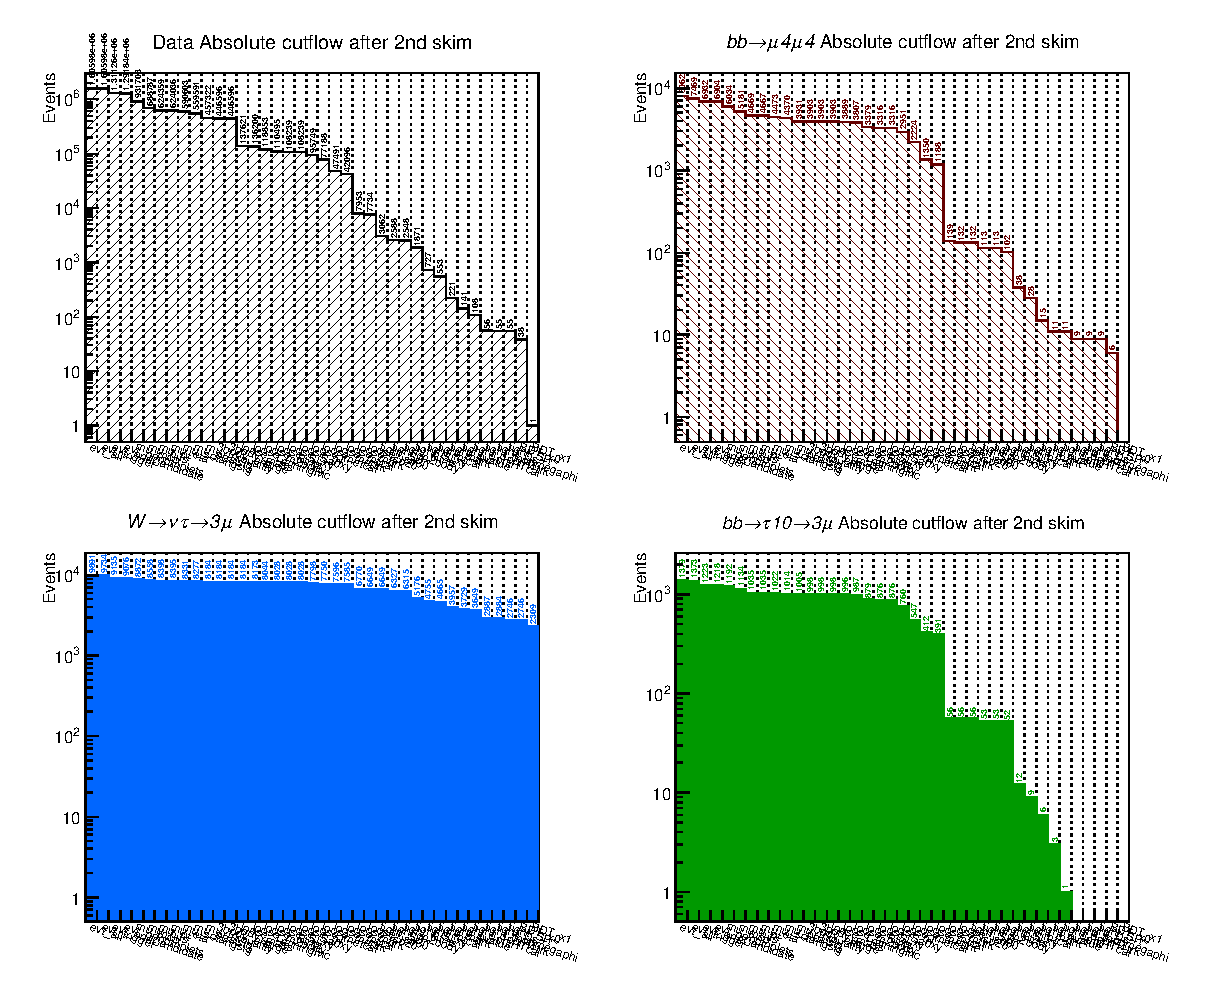
\includegraphics[scale=0.5]{cutflow.muons.mva.all.eps}};
\end{tikzpicture}
\end{columns}
\end{frame}
\Sec{Weighted cutflow for 20~fb$^{-1}$}{Weighted cutflow for 20~fb$^{-1}$}{sec:weightedcutflow}
\begin{frame}{}
\hspace*{-1cm}
\begin{columns}
\column{12cm}
\begin{tikzpicture}
	\node{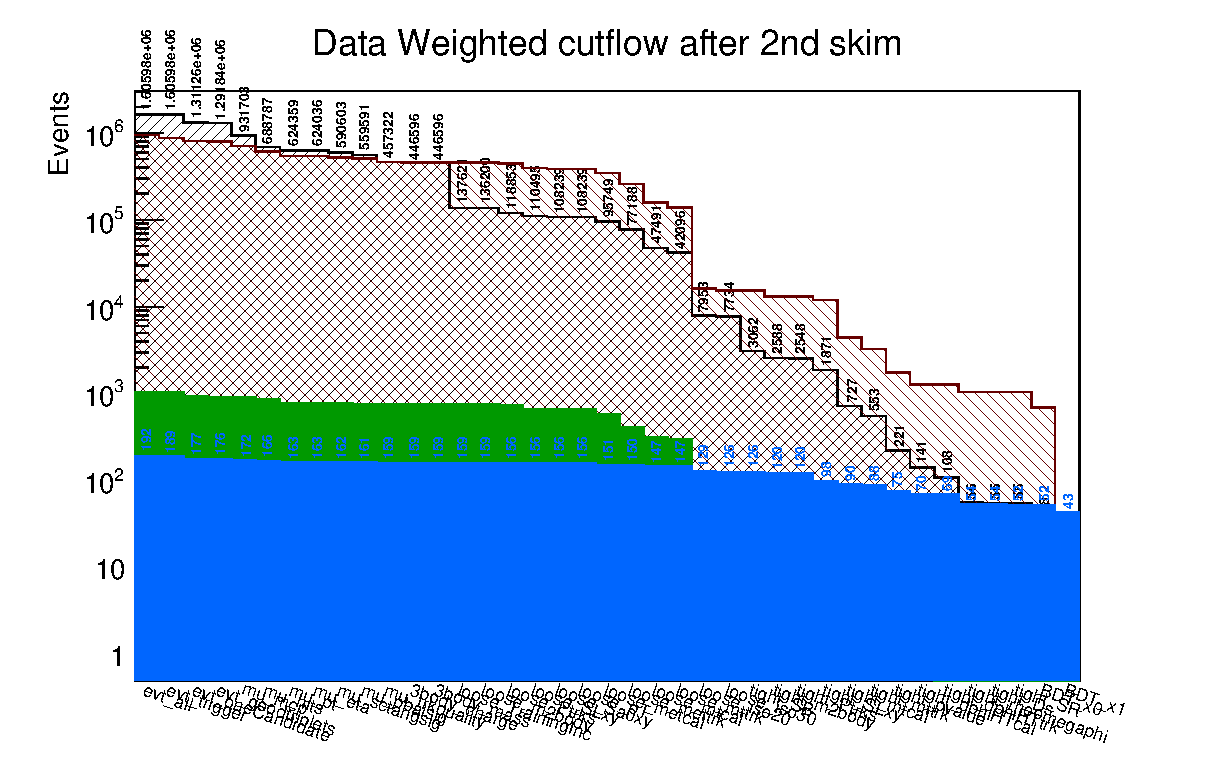
\includegraphics[scale=0.6]{cutflow.muons.mva.weighted.eps}};
\end{tikzpicture}
\end{columns}
\end{frame}
\Sec{Normalized cutflow}{Normalized cutflow}{sec:normalizedcutflow}
\begin{frame}{}
\hspace*{-1cm}
\begin{columns}
\column{12cm}
\begin{tikzpicture}
	\node{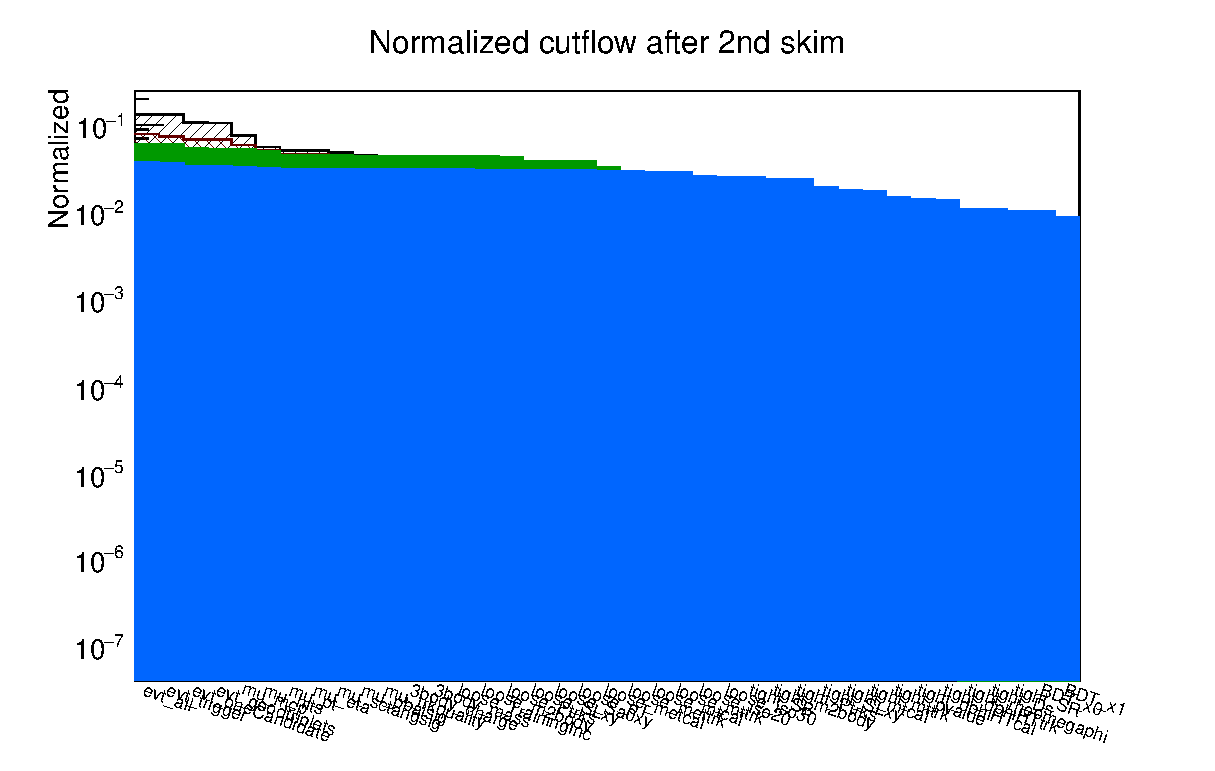
\includegraphics[scale=0.6]{cutflow.muons.mva.normalized.eps}};
\end{tikzpicture}
\end{columns}
\end{frame}
\Sec{Analysis level}{Analysis level}{sec:analysislevel}
\begin{frame}{}
\vspace*{-0.3cm}
\hspace*{+1.5cm}
\begin{columns}
\column{12cm}
\hspace*{+1cm}
\begin{tikzpicture}
\node[scale=0.325]{
\begin{tabular}[t]{l|rr|rr|rr}
	\hline\hline
	Cut	& $W\to\nu\tau\to 3\mu$ & Efficiency & $bb\to\mu 4\mu 4$ & Rejection ($1-\epsilon$) & Data & Rejection \\[3pt]
	\hline
	All - after skim2 &9891 &-- &8062 &-- &1605975 &-- \\[3pt]
	Trigger - after skim2 &9734 &98.41\% &7469 &7.36\% &1605975 &0.00\% \\[3pt]
	Trigger - after skim2 &9135 &93.85\% &6932 &7.19\% &1311256 &18.35\% \\[3pt]
	Category is $3\mu$ or $2\mu+1\tpa$ &9076 &99.35\% &6904 &0.40\% &1291836 &1.48\% \\[3pt]
	\hline
	Std. MCP ID-hits cut &8872 &97.75\% &6034 &12.60\% &931703 &27.88\% \\[3pt]
	TRT+MS hits &8558 &96.46\% &5181 &14.14\% &688787 &26.07\% \\[3pt]
	$p_T^{1,2,3}>5.5,3.5,2.5$~GeV &8398 &98.13\% &4669 &9.88\% &624359 &9.35\% \\[3pt]
	$|\eta|<2.5$ &8395 &99.96\% &4667 &0.04\% &624036 &0.05\% \\[3pt]
	Muon scattering angle sig.$<5$ &8331 &99.24\% &4473 &4.16\% &590603 &5.36\% \\[3pt]
	Muon momentum balance sig.$<3$ &8277 &99.35\% &4370 &2.30\% &559591 &5.25\% \\[3pt]
	\tpa track-fit $\pvalue>0.01$ &8184 &98.88\% &3931 &10.05\% &457322 &18.28\% \\[3pt]
	\hline
	$|\Sigma Q_{3{\rm body}}|=1|LINE$ &8184 &100.00\% &3903 &0.71\% &446596 &2.35\% \\[3pt]
	$\mthreebody<5$~GeV &8184 &100.00\% &3903 &0.00\% &446596 &0.00\% \\[3pt]
	Training+SB+Blinded: \TrainingRegion~MeV &8184 &100.00\% &3903 &0.00\% &137621 &69.18\% \\[3pt]
	$\mOSa>220$~MeV, $\mOSb>220$~MeV and $\mSS>220$~MeV &8173 &99.87\% &3889 &0.36\% &136200 &1.03\% \\[3pt]
	$\ptrks>10^{-9}$ &8044 &98.42\% &3807 &2.11\% &118853 &12.74\% \\[3pt]
	$-10<\SLxy<50$ &8028 &99.80\% &3379 &11.24\% &110495 &7.03\% \\[3pt]
	$\Sazeroxy<25$ &8028 &100.00\% &3316 &1.86\% &108239 &2.04\% \\[3pt]
	$\pTthreebody>10$~GeV &8028 &100.00\% &3316 &0.00\% &108239 &0.00\% \\[3pt]
	$10<\calomet<250$~GeV &7798 &97.14\% &2951 &11.01\% &95749 &11.54\% \\[3pt]
	$10<\trackmet<250$~GeV &7750 &99.38\% &2224 &24.64\% &77188 &19.39\% \\[3pt]
	$\mTcalo>20$~GeV &7596 &98.01\% &1350 &39.30\% &47491 &38.47\% \\[3pt]
	$\mTtrack>20$~GeV &7585 &99.86\% &1188 &12.00\% &42096 &11.36\% \\[3pt]
	$\isoTwenty<0.3$ &6770 &89.26\% &139 &88.30\% &7953 &81.11\% \\[3pt]
	$\isoThirty<1$ &6649 &98.21\% &132 &5.04\% &7734 &2.75\% \\[3pt]
	\hline
	SB: \SidebandLeftBrackets+\SidebandRightBrackets~MeV &6649 &100.00\% &132 &0.00\% &3062 &60.41\% \\[3pt]
	$\mOSa>300$~MeV, $\mOSb>300$~MeV and $\mSS>300$~MeV &6327 &95.16\% &113 &14.39\% &2588 &15.48\% \\[3pt]
	$\ptrks>8\times 10^{-9}$ &6315 &99.81\% &113 &0.00\% &2548 &1.55\% \\[3pt]
	$1<\SLxy<50$ &5176 &81.96\% &102 &9.73\% &1871 &26.57\% \\[3pt]
	$\mTcalo>45$~GeV &4755 &91.87\% &38 &62.75\% &727 &61.14\% \\[3pt]
	$\mTtrack>45$~GeV &4665 &98.11\% &28 &26.32\% &553 &23.93\% \\[3pt]
	$\pvalue>0.2$ &3957 &84.82\% &15 &46.43\% &221 &60.04\% \\[3pt]
	$\dphiHmetcalo>2$ &3729 &94.24\% &11 &26.67\% &141 &36.20\% \\[3pt]
	$\dphiHmettrack>2$ &3649 &97.85\% &11 &0.00\% &108 &23.40\% \\[3pt]
	\rhoomega and $\phi$ veto &2887 &79.12\% &9 &18.18\% &56 &48.15\% \\[3pt]
	\Ds veto &2884 &99.90\% &9 &0.00\% &55 &1.79\% \\[3pt]
	\hline
	SR: \SignalRegion~MeV &2746 &95.21\% &9 &0.00\% &55 &0.00\% \\[3pt]
	\hline
	BDT score $x>\xzrovalue$ &2746 &100.00\% &6 &33.33\% &38 &30.91\% \\[3pt]
	\hline
	BDT score $x>\xoptvalue$ &2309 &84.09\% &0 &100.00\% &1 &97.37\% \\
	\hline
	\hline\hline
\end{tabular}};
\end{tikzpicture}
\end{columns}
\end{frame}
\end{document}
